\chapter{Evaluation Model B: Two-Dimensional Gaze-Weighted Evaluation}
\label{ch:model-b}

\section{Methodology change}
On 2026-09-13, following an explicit project decision, gaze-weighted (time-weighted
ghost/blind fraction) evaluation was promoted from a secondary, comparison-only
analysis to this project's \textbf{primary} array-safety standard, judged more
realistic than a pure worst-case-across-every-tested-gaze-angle criterion (source:
\texttt{Array\_Design/array\_geometry\_lab/GAZE\_WEIGHTED\_APPROACH.md}, ``UPDATE,
2026-09-13'' section, and
\texttt{array\_data/evaluation\_results/TIMELINE.txt}, both verified present, mtime
2026-09-13 14:10--14:11). Model~A (Chapter~\ref{ch:model-a}) was not deleted or edited
-- it remains valid, fully reported data -- but is no longer this project's headline
answer.

\section{Full-azimuth, gaze-time-weighted sampling}
\label{sec:model-b-method}
Model B removes Model A's single-axis limitation (Section~\ref{sec:model-a-limitation})
directly: for each of 26 eccentricity bins (bin centers $0.5^\circ$ to $27.0^\circ$,
weighted by an empirically measured eccentricity distribution -- \%
of viewing time per bin, summing to $100.0\%$, cumulative $51.61\%$ by $6^\circ$ and
$95.27\%$ by $17^\circ$, checked to satisfy both cumulative checkpoints before any sweep
runs), the pupil is sampled at $N_\theta=36$ azimuths uniformly around the full circle,
using the same validated radial-shift magnitude (Equation~\ref{eq:pupil-shift}) applied
in an arbitrary direction: $\mathrm{pupil\_center}=(R\cos\theta,R\sin\theta)$.

\begin{keybox}{The $27^\circ$ bin is explicitly flagged as extrapolated}
The eccentricity distribution's own highest bin is centered at $27^\circ$ (0.58\% of
viewing time), \textbf{outside} \texttt{vignetting\_overlap.py}'s own stated small-angle
validity range for the pupil-shift formula, $|\varphi|\le25^\circ$. The formula does not
numerically diverge there -- it is still evaluated, per the source module's own
docstring, ``the formula doesn't blow up... every caller that reports a number must
check and flag this, not silently trust it'' -- and this paper does exactly that: every
number in this chapter that includes the $27^\circ$ bin is extrapolated beyond the
formula's own validated range, at only 0.58\% total weight, and is flagged here rather
than silently trusted.
\end{keybox}

At each active hole, the illuminated area is the exact overlap area of
Equation~\ref{eq:overlap}; a hole counts as \emph{active} when its own illuminated
fraction exceeds $0.5$ (\texttt{margins/active\_pairs.py}'s
\texttt{DEFAULT\_ACTIVE\_FRAC\_THRESHOLD}, reused unmodified here, so ``ghosting'' means
the identical thing in Model~B as in Model~A). \textit{Blind} is total illuminated area
exactly zero, time-weighted across every sampled $(\varphi,\theta)$ pair, giving
\texttt{time\_weighted\_blind\_pct} and \texttt{time\_weighted\_ghost\_pct} per candidate
(source: \texttt{array\_calculation/compute\_gaze\_weighted\_metrics.py}, verified read
directly).

\section{Adding a hard blindness gate}
\label{sec:blindness-gate}
The primary ranking rule (\texttt{comparison\_metric/primary\_ranking\_gaze\_weighted.py})
hard-gates any candidate with \texttt{time\_weighted\_blind\_pct} above a tolerance,
then minimizes \texttt{time\_weighted\_ghost\_pct} among survivors.

\begin{warnbox}{A strict 0\% blindness gate was tried first and rejected -- checked, not assumed}
A strict $0\%$-blind gate produces a sharp cliff at $M=6$D/$8$D: it forces ghost
percentages up to 27--30\%, because every genuinely-zero-blind candidate at those $M$
carries real ghost, while the best hexagonal candidates there carry only a small
0.12--0.33\% blind time. This is the same ``margin-vs-zero'' failure mode Model~A's own
audit fix (Section~\ref{sec:three-gates}) had already diagnosed once before, in a
different context. A $1.0\%$ tolerance was used instead, which clears every existing
winner's own blind percentage with headroom and produces the identical family choices
as the earlier ungated ranking (hexagonal $M=1$--$6$, square $M=0/8$/global) -- the gate
exists to prevent a \emph{future} re-run from silently accepting a degenerate design, it
did not have to override anything in the current result set.
\end{warnbox}

\begin{figure}[htbp]
\centering
\begin{minipage}{0.32\textwidth}\centering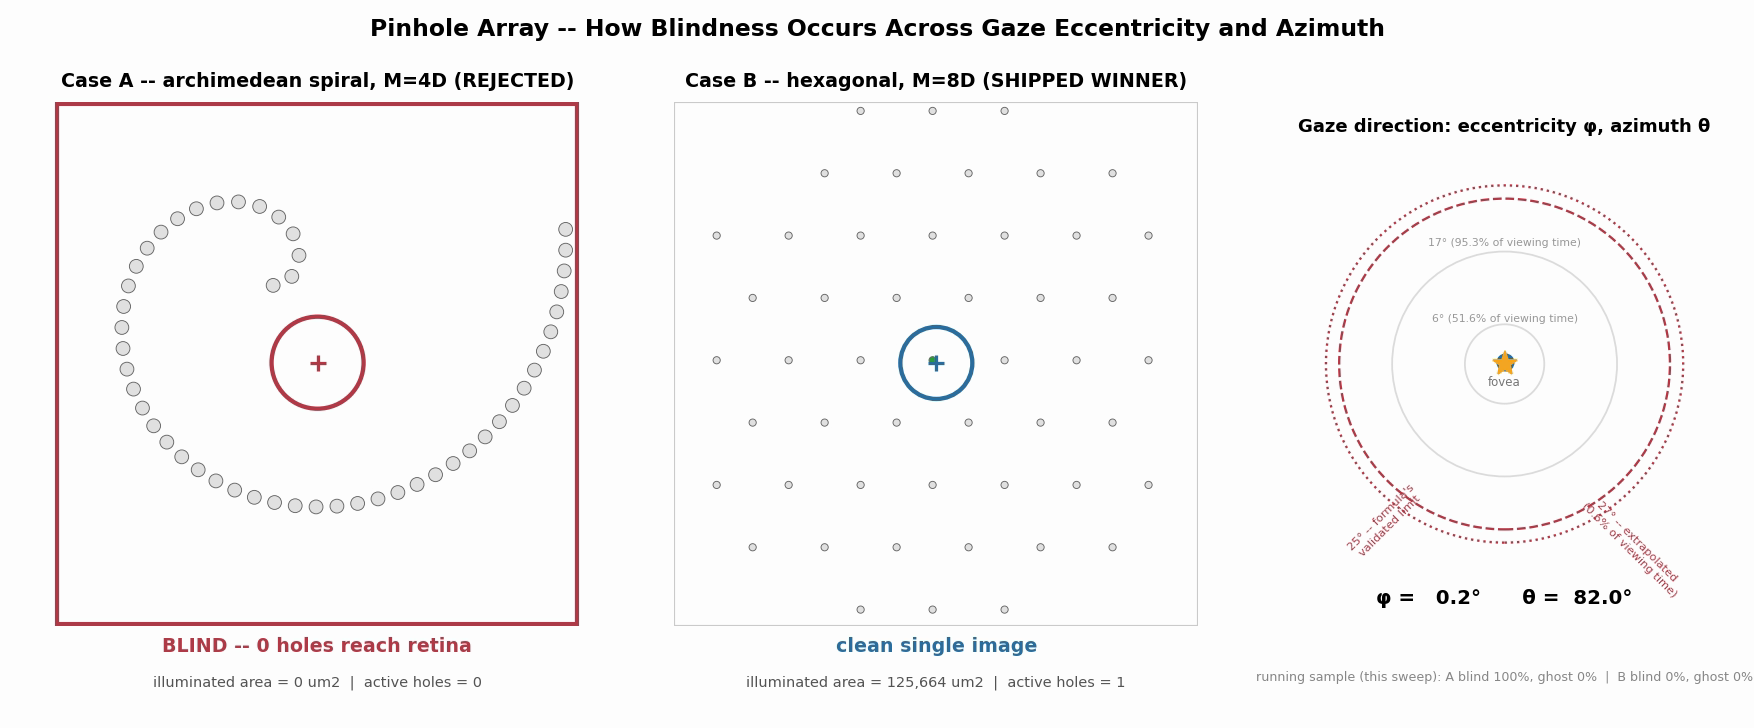
\includegraphics[width=\textwidth]{figures/blindness_frame_blind.png}\end{minipage}\hfill
\begin{minipage}{0.32\textwidth}\centering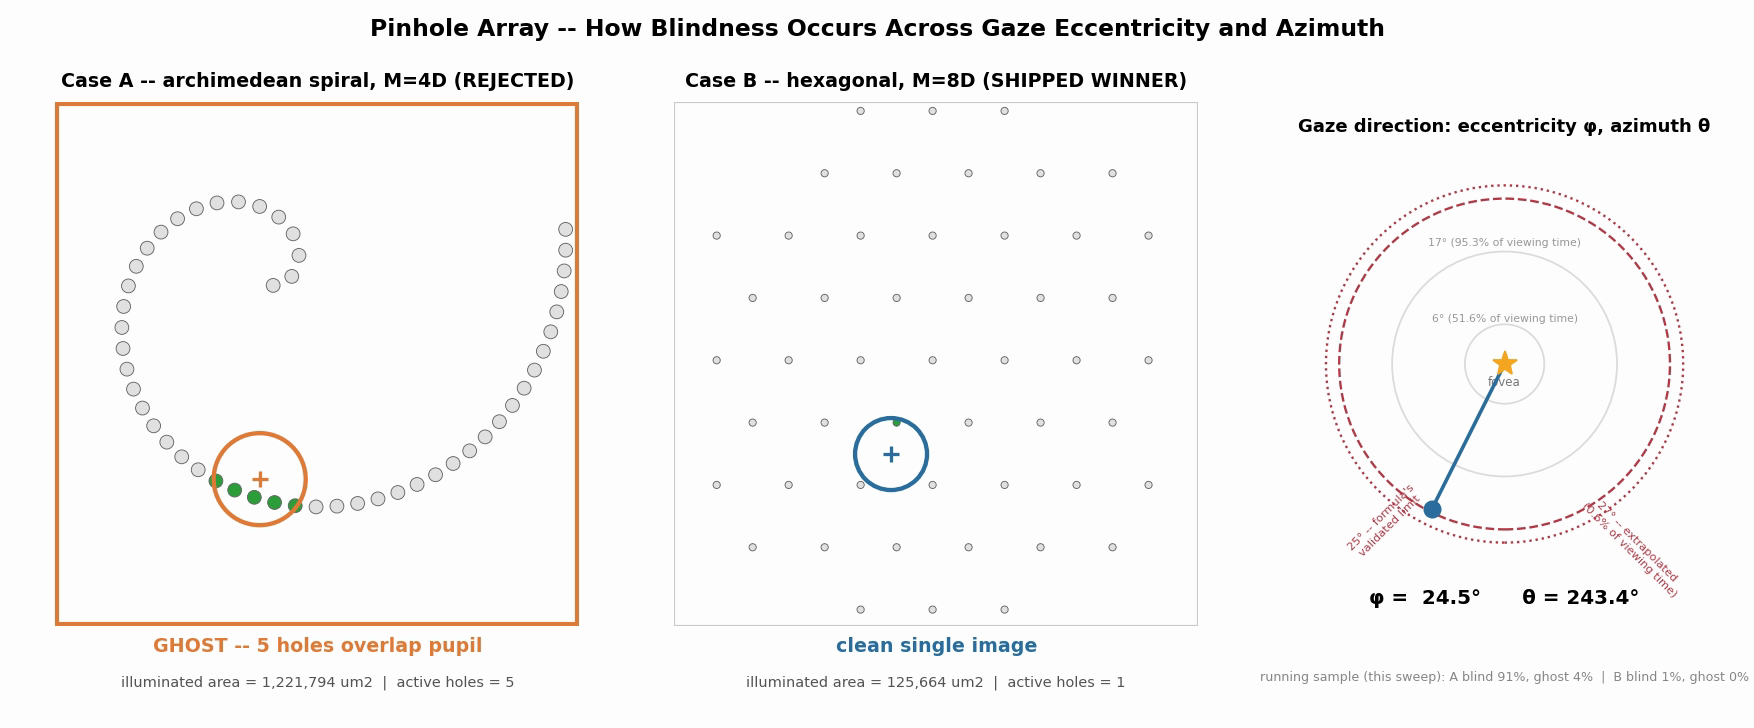
\includegraphics[width=\textwidth]{figures/blindness_frame_ghost.png}\end{minipage}\hfill
\begin{minipage}{0.32\textwidth}\centering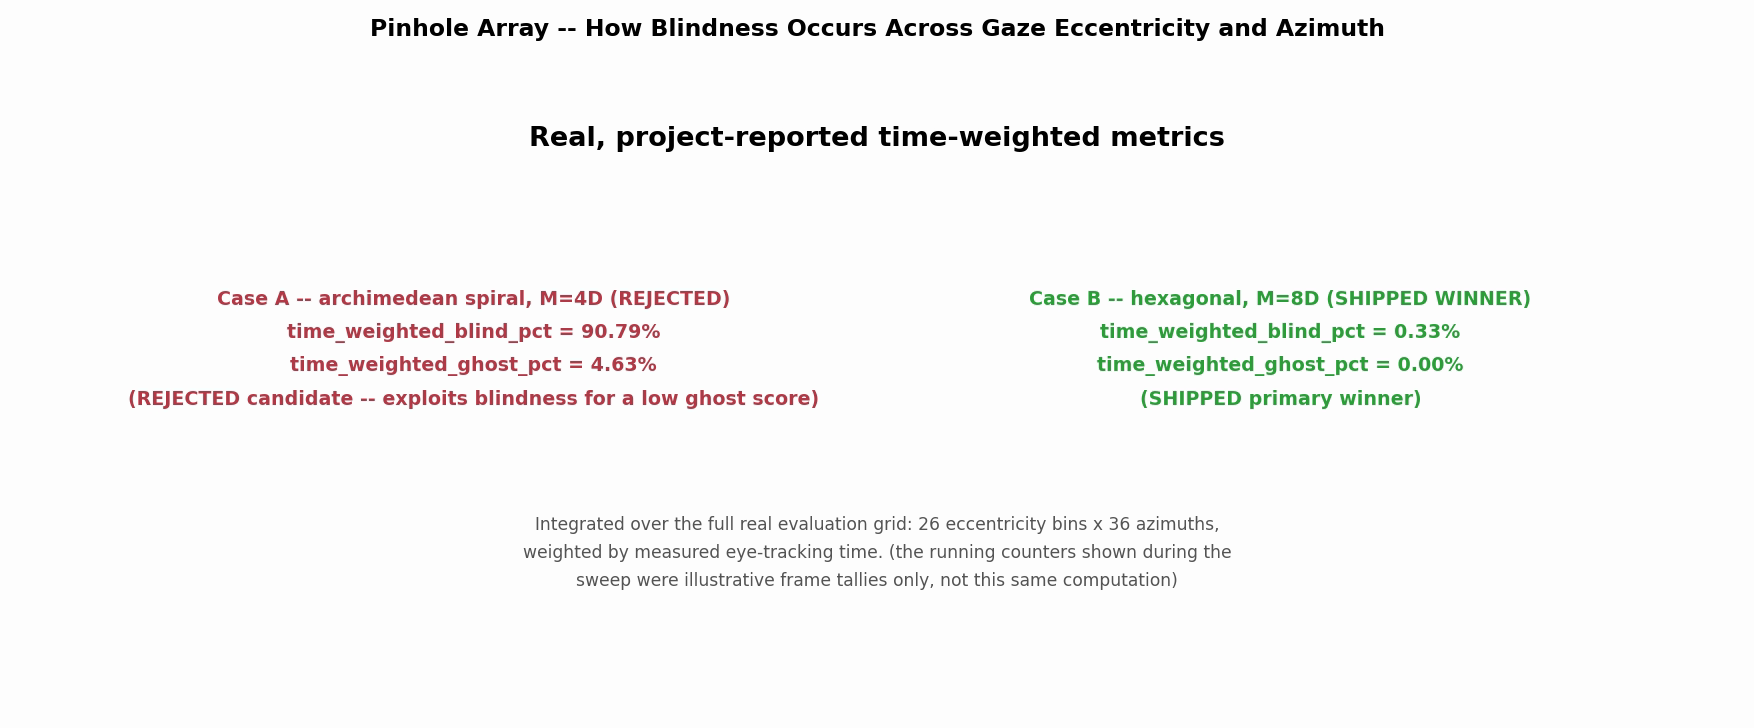
\includegraphics[width=\textwidth]{figures/blindness_frame_clean.png}\end{minipage}
\caption{All three states this section's gate distinguishes, shown side by side for
the same two real candidates swept through the identical $(\varphi,\theta)$ gaze path
-- Case A: \texttt{archimedean\_spiral}, $M=4$D (a real, rejected candidate,
$90.79\%$ time-weighted blind); Case B: the shipped hexagonal $M=8$D primary winner
($0.33\%$ blind). Left: Case~A \textbf{BLIND} ($\varphi=0.2^\circ,\theta=82.0^\circ$,
0 holes reach the retina). Middle: Case~A \textbf{GHOST} (5 simultaneously active
holes at $\varphi=24.5^\circ,\theta=243.4^\circ$) -- note the images coincide near
$\varphi=0$ but a real ghost-separation only appears at higher $\varphi$, consistent
with $\Delta r(s,M)=sM/(P_0-M)$ vanishing only at $M=0$, not at $\varphi=0$. Right:
both cases \textbf{clean}. Frames extracted via \texttt{ffmpeg} from
\texttt{Array\_Design/array\_geometry\_lab/blindness\_mechanism\_animation/}
\texttt{blindness\_mechanism\_animation.mp4} (mtime 2026-09-16 12:58); the underlying
simulation reuses \texttt{engine/vignetting\_overlap.py}'s validated overlap-area
formula and \texttt{engine/ghost\_formula.py}'s validated separation formula
unmodified -- the same two functions used throughout Chapter~\ref{ch:array-theory}.}
\label{fig:blindness-states}
\end{figure}

\section{Current results}
\label{sec:model-b-results}
Source: \texttt{Array\_Design/array\_geometry\_lab/array\_data/evaluation\_results/PRIMARY\_WINNER\_PER\_M.csv},
mtime 2026-09-13 14:10 (the most recent evaluation-results file in its directory as of
this writing; see Chapter~\ref{ch:provenance}).
\begin{center}
\begin{tabular}{cccccc}
\toprule
$M$ (D) & Family & $a_{\mathrm{hole}}$ ($\mu$m) & $N$ & Blind \% & Ghost \% \\
\midrule
0 & square & 2000 & 20 & 0.00 & 0.00 \\
1 & hexagonal & 1250 & 20 & 0.00 & 0.00 \\
2 & hexagonal & 750 & 20 & 0.00 & 0.00 \\
3 & hexagonal & 750 & 20 & 0.00 & 0.00 \\
4 & hexagonal & 600 & 20 & 0.00 & 0.00 \\
5 & hexagonal & 600 & 20 & 0.00 & 0.00 \\
6 & hexagonal & 500 & 100 & 0.12 & 0.00 \\
8 & hexagonal & 400 & 50 & 0.33 & 0.00 \\
\bottomrule
\end{tabular}
\end{center}
Hexagonal packing wins six of eight tested myopia powers; square wins at $M=0$ and the
global (worst-case-across-$M$) scope. Every winning design achieves genuine $0.00\%$
ghost under realistic, time-weighted gaze -- not merely a structural worst-case
guarantee -- and the only two nonzero blind percentages in the table (0.12\%, 0.33\%)
are both well inside the $1.0\%$ gate of Section~\ref{sec:blindness-gate}.

\section{Why hexagonal: the physical intuition}
\label{sec:hex-intuition}
As the eye rotates by $\varphi$, the pupil shifts in \emph{some} azimuth $\theta$ that
could, physically, be any direction the wearer happens to look. A safe array needs small
gaps between holes in every direction, not only a single favoured axis. Three properties
of a hexagonal lattice matter here, all standard results:

\begin{enumerate}
\item \textbf{Densest possible 2D point packing.} Hexagonal packing achieves packing
density $\pi/(2\sqrt3)\approx0.9069$, provably optimal (the honeycomb conjecture) -- for
a given minimum safe pitch, it fits the most holes into that pitch.
\item \textbf{Maximum rotational symmetry for a periodic lattice.} A hexagonal lattice
has 6-fold rotational symmetry -- the \emph{maximum} any periodic 2D lattice can have at
all, by the crystallographic restriction theorem (only 2-, 3-, 4-, and 6-fold rotations
are compatible with translational periodicity). This makes the gap structure between
holes nearly isotropic: it matters comparatively little which azimuth the pupil happens
to shift toward.
\item \textbf{Regular-hexagon Voronoi cells.} The Voronoi cell of a hexagonal lattice
point is a regular hexagon -- the polygon that best approximates a circle while still
tiling the plane with no gaps -- directly minimizing the worst-case distance from any
pupil position to its nearest hole, uniformly in every direction.
\end{enumerate}

A square lattice, by contrast, has only 4-fold symmetry: its diagonal ($45^\circ$)
nearest-neighbor distance is $\sqrt2\times$ its axis-aligned nearest-neighbor distance --
a real, quantifiable weak direction. This is exactly the mechanism behind the concrete
ring-family blackout of Section~\ref{sec:model-a-limitation}: a ring-based design's holes
exist only at discrete angular positions (a fixed \texttt{holes\_per\_ring0} count), with
real angular gaps between them that a single-axis test can miss entirely.

\begin{figure}[htbp]
\centering
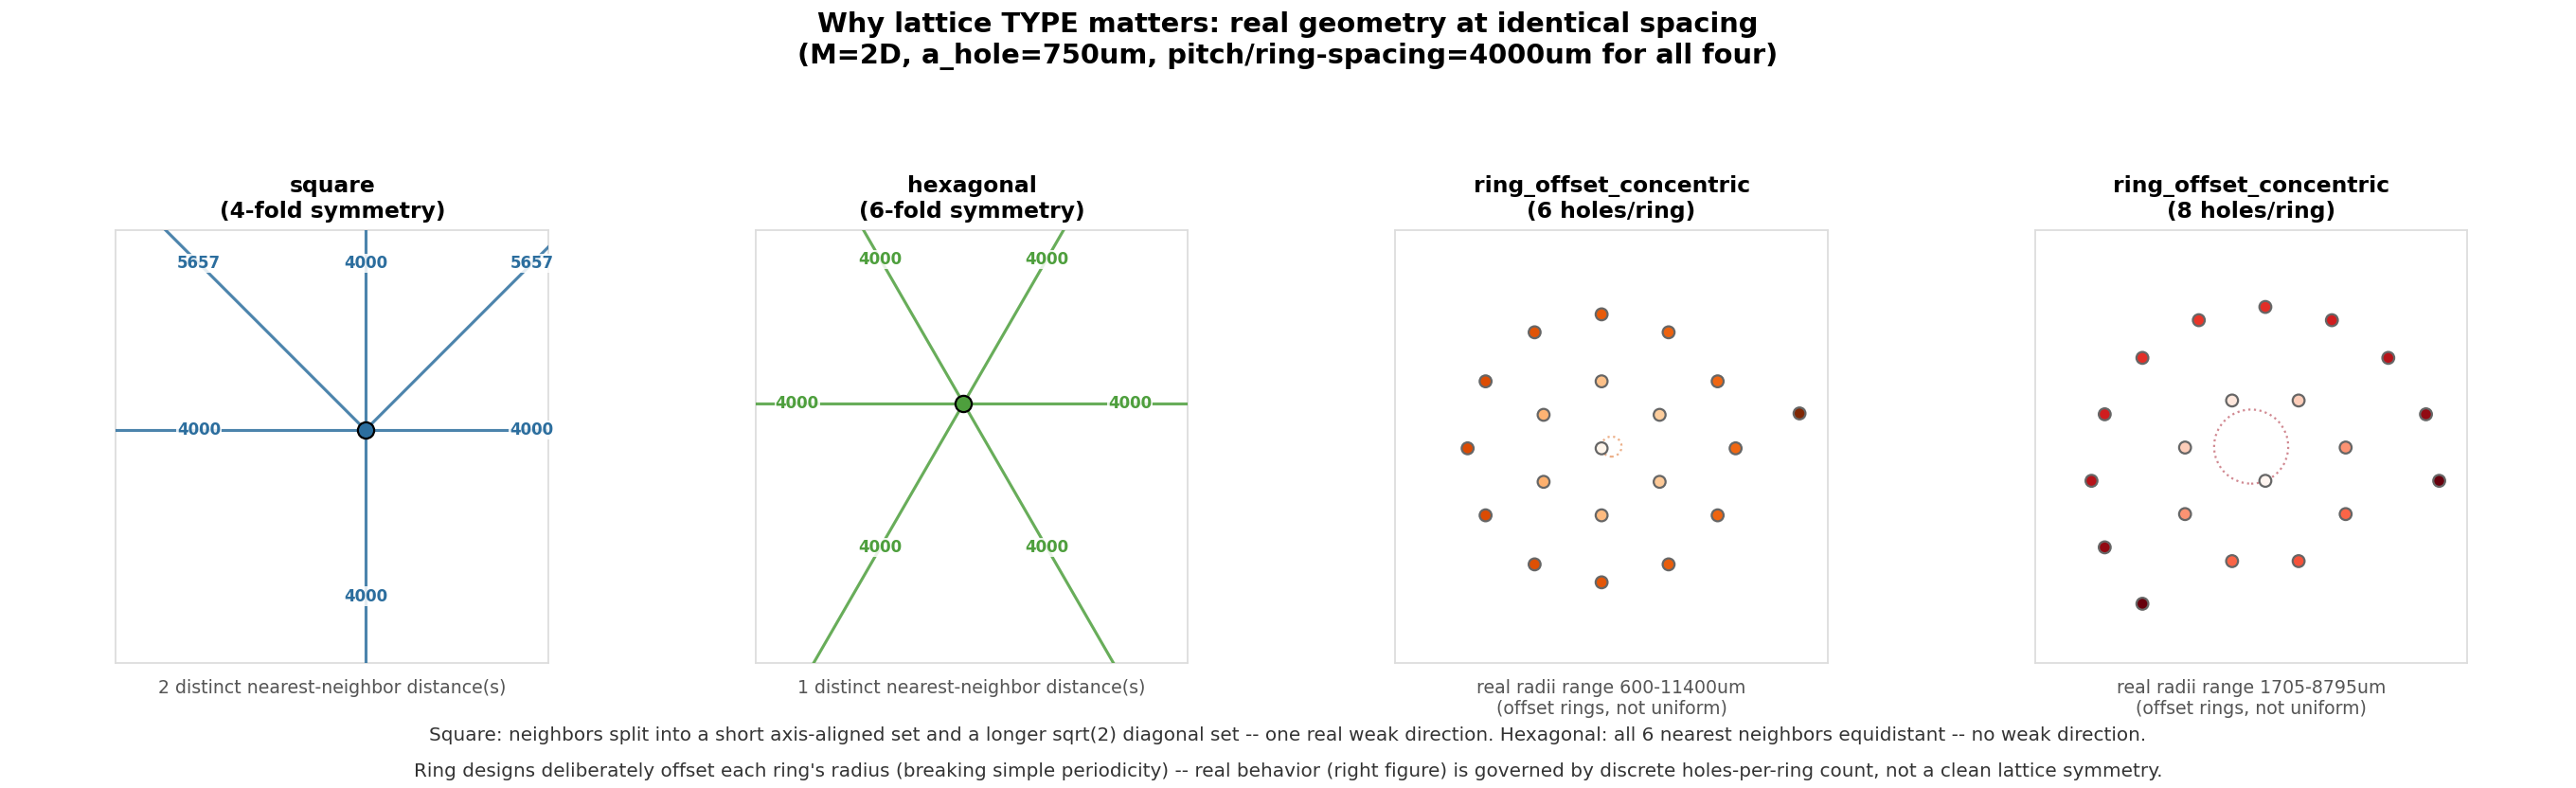
\includegraphics[width=0.95\textwidth]{figures/geometry_intuition_structure.png}
\caption{Real regenerated nearest-neighbor structure at identical spacing
(pitch/ring-spacing $=4000\,\mu$m, $a_{\mathrm{hole}}=750\,\mu$m, $M=2$D). Square: two
distinct nearest-neighbor distances, 4000 and $5657\,\mu$m ($=4000\sqrt2$, confirming the
diagonal weak direction exactly). Hexagonal: one distinct distance, all six neighbors
equidistant. Ring designs (6 and 8 holes/ring): genuinely offset, non-uniform ring
radii, not a simple lattice -- shown as real coordinate scatter rather than forced into
the same distance-count framing. Source: this analysis, regenerated directly from
\texttt{array\_calculation/degeneracy\_filter.py}'s own generator functions; see
Chapter~\ref{ch:provenance}.}
\label{fig:geom-structure}
\end{figure}

\begin{figure}[htbp]
\centering
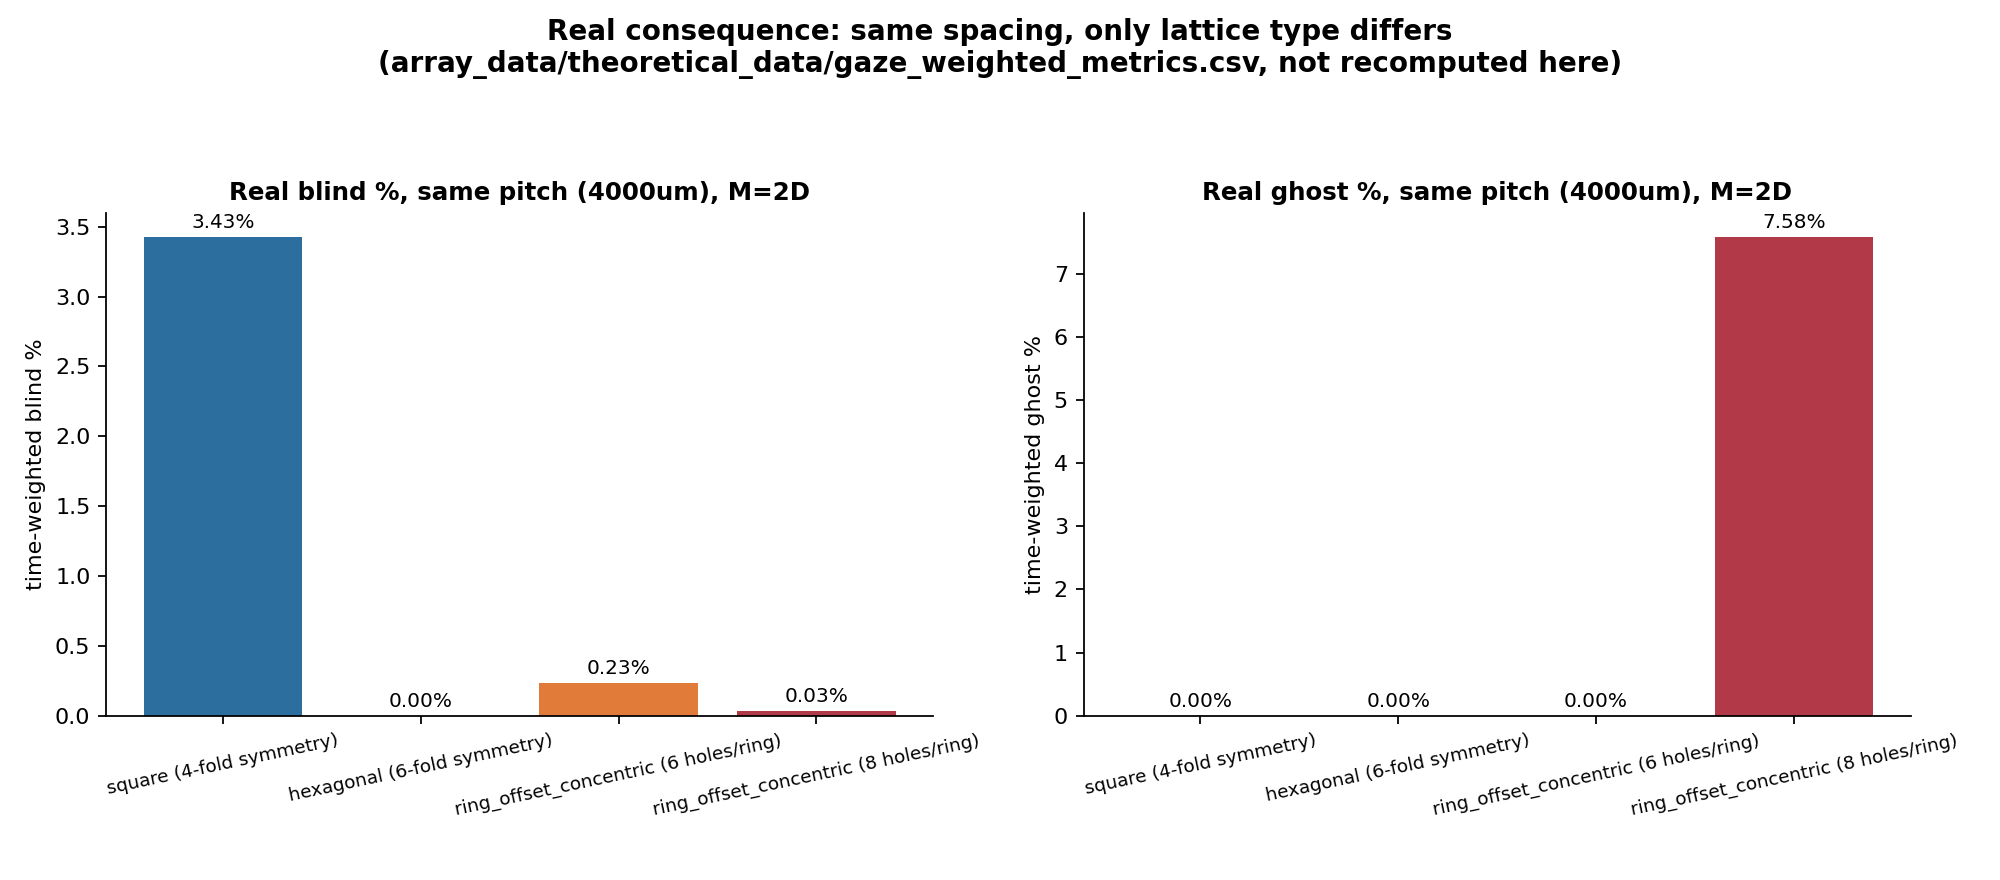
\includegraphics[width=0.85\textwidth]{figures/geometry_intuition_real_consequence.png}
\caption{Real, already-computed gaze-weighted blind\%/ghost\% for the same four
matched-spacing designs as Figure~\ref{fig:geom-structure}, read directly from
\texttt{array\_data/theoretical\_data/gaze\_weighted\_metrics.csv} (not recomputed for
this figure). Hexagonal is the only design with $0.00\%$ on both axes simultaneously;
the ring-of-8 design trades blind\% for a real $7.58\%$ ghost fraction -- the discrete
angular-gap tension (Section~\ref{sec:blinding}) hexagonal packing avoids by being
simultaneously dense and well-separated in every direction.}
\label{fig:geom-consequence}
\end{figure}

\section{Predicted acuity is identical across every evaluation model}
\label{sec:model-comparison-table}
Because every array evaluation model chooses its aperture from the same
acuity-optimum map (Chapter~\ref{ch:model-comparison}, Table~\ref{tab:predicted-acuity})
before deciding geometry, all six live evaluation models tested in this project's
own analysis (Model A / \texttt{FINAL\_WINNER\_PER\_M.csv}; Model~B /
\texttt{PRIMARY\_WINNER\_PER\_M.csv}; the ungated gaze-weighted ranking; density-only
Metric~1; and two effective-density variants) produce \textbf{numerically identical}
predicted LogMAR per myopia power -- confirmed directly, not assumed, by looking up
each model's own chosen aperture in the corrected acuity sweep
(\texttt{new\_sweeps/acuity\_sweep\_stage4.csv}) and finding zero deviation across all
six (Chapter~\ref{ch:model-comparison}). Choice of evaluation model changes
\emph{safety} (ghost/blind risk), never predicted optical acuity.
